\documentclass{article}
\usepackage[utf8]{inputenc}
\usepackage{graphicx}

\title{CARA MERANCANG DAN MEMBUAT APLIKASI PENCUCIAN MOBIL PADA APEX ONLINE}
\author{Dimas Aqila Maulana (1184081)}
\date{19 December 2019}

\begin{document}

\maketitle

\section{Rancangan Database di Apex Online}
\begin{itemize}
\item Hal yang harus dibuat pertama ialah tabel-tabel yang nanti akan dimasukan ke aplikasi tersebut, tentunya yang berkaitan dengan apa yang akan kita buat, pertama marilah kita buat akun oracle apex online dan login ke oracle tersebut seperti pada gambar \ref{login}

\begin{figure}[!htbp]
    \centering
    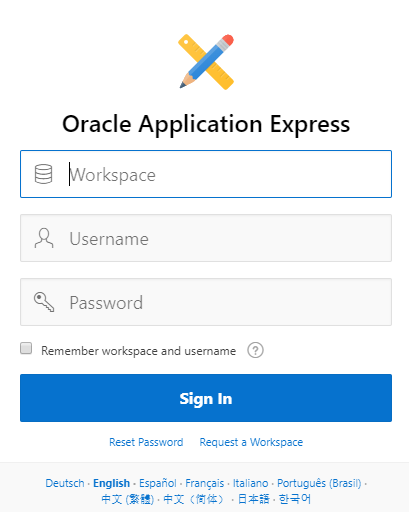
\includegraphics[scale=0.63]{figures/10.PNG}
    \caption{Login Apex Online}
    \label{login}
\end{figure}

\item Lalu setelah login pilih menu SQL workshop, disini berguna untuk menjalankan query-query yang diperlukan untuk membuat tabel tersebut disini saya membuat tabel pelanggan dimana nik dijadikan primary key, kode jenis cuci sebagai foreign key dan kode pencuci sebagai foreign key juga seperti pada gambar \ref{menu}
\begin{figure}[!htbp]
    \centering
    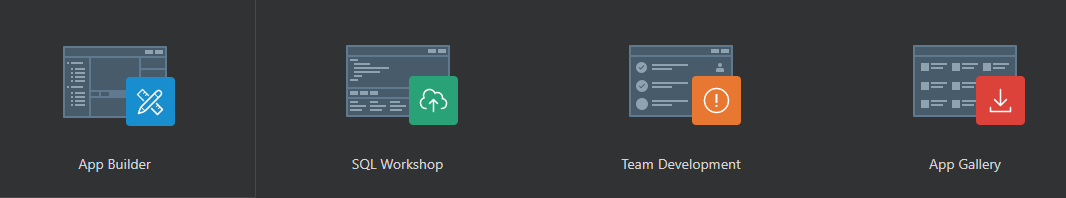
\includegraphics[scale=0.5]{figures/11.PNG}
    \caption{Menu Oracle Apex}
    \label{menu}
\end{figure}
\item Setelah terbuka ketikkan query sebagai berikut agar dapat membuat tabel di database tersebut seperti pada gambar \ref{tabel1}
\begin{figure}[!htbp]
    \centering
    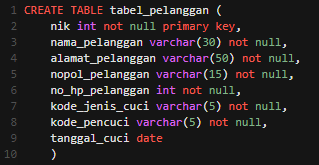
\includegraphics[scale=1]{figures/1.PNG}
    \caption{Tabel Pelanggan}
    \label{tabel1}
\end{figure}
\item Buat juga tabel cuci yang berfungsi sebagai relasi tabel pelanggan, disini saya membuat kode jenis cuci sebagai primary key dari tabel cuci menggunakan tipe data varchar karena agar bisa memasukkan huruf dan angka secara berurutan seperti pada gambar \ref{tabel2}
\begin{figure}[!htbp]
    \centering
    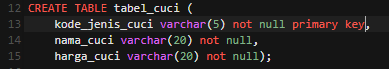
\includegraphics[scale=1]{figures/2.PNG}
    \caption{Tabel Cuci}
    \label{tabel2}
\end{figure}
\item Disini saya juga membuat tabel pencuci yang bertujuan untuk mengetahui siapa orang yang mencuci mobil pelanggan tersebut, saya menjadikan kode pencuci sebagai primary keynya seperti pada gambar \ref{tabel3}
\begin{figure}[!htbp]
    \centering
    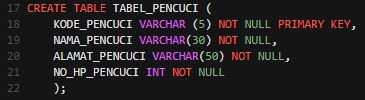
\includegraphics[scale=1.2]{figures/3.PNG}
    \caption{Tabel Pencuci}
    \label{tabel3}
\end{figure}
\item Lalu ada tabel Log pelanggan yang berfungsi untuk merecord data pelanggan yang di insert, delete, dan update, saya hanya menampilkan yang penting saja dari tabel-tabel diatas seperti nik dan nama pelanggan, tanggal dan keterangan digunakan untuk merecord seperti pada gambar \ref{tabel4}
\begin{figure}[!htbp]
    \centering
    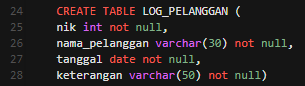
\includegraphics[scale=1.3]{figures/4.PNG}
    \caption{Log Pelanggan}
    \label{tabel4}
\end{figure}
\item Setelah semua tabel sudah dibuat, kita akan merelasikan semua tabel yang berhubungan seperti pada tabel pelanggan berelasi dengan tabel cuci dan tabel pencuci, disini kita menggunakan query seperti pada gambar \ref{tabel5}
\begin{figure}[!htbp]
    \centering
    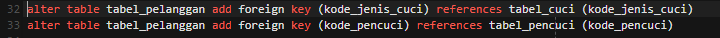
\includegraphics[scale=0.65]{figures/5.PNG}
    \caption{Membuat Foreign Key}
    \label{tabel5}
\end{figure}
\item Disini kita sampai pada tahap pembuatan query trigger yang berfungsi sebagai insert, update dan delete dan akan terecord apabila ada data yang diubah, akan ada recordnya pada trigger tersebut, saya membuat trigger pada tabel pelanggan, querynya seperti pada gambar \ref{trigger1}
\begin{figure}[!htbp]
    \centering
    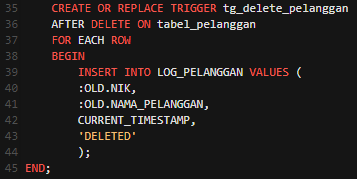
\includegraphics[scale=0.9]{figures/6.PNG}
    \caption{Trigger Delete}
    \label{trigger1}
\end{figure}
\item Setelah delete kita buat trigger insert yang berfungsi untuk merecord data yang akan dimasukkan pada tabel pelanggan querynya juga tentu berbeda seperti new.nik karena insert berupa data baru tidak seperti old.nik yang merupakan data lama seperti pada gambar \ref{trigger2}
\begin{figure}[!htbp]
    \centering
    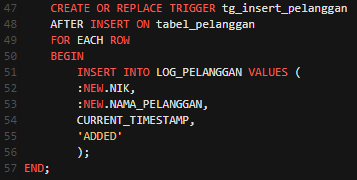
\includegraphics[scale=0.9]{figures/7.PNG}
    \caption{Trigger Insert}
    \label{trigger2}
\end{figure}
\item Trigger update sama seperti trigger insert hanya beda saat keterangannya saja seperti pada gambar \ref{trigger3}
\begin{figure}[!htbp]
    \centering
    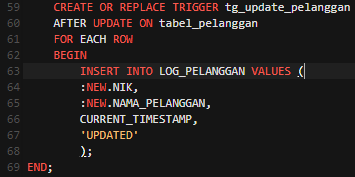
\includegraphics[scale=0.9]{figures/8.PNG}
    \caption{Trigger Update}
    \label{trigger3}
\end{figure}
\item Sesudah membuat semua tabel dan trigger tersebut, selanjutnya adalah membuat view yang bertujuan untuk memanggil semua tabel yang sudah dimasukkan kepada query view tersebut, contohnya saya memasukkan ke tiga tabel tersebut kedalam view agar dapat terlihat semuanya seperti pada gambar \ref{view}
\begin{figure}[!htbp]
    \centering
    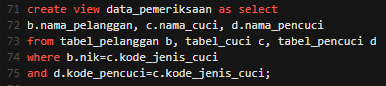
\includegraphics[scale=0.9]{figures/9.PNG}
    \caption{View}
    \label{view}
\end{figure}
\end{itemize}

\section{Pembuatan Aplikasi Oracle Apex}
\begin{itemize}
\item Pada menu oracle apex pilih menu app builder lalu klik create dan buat new application seperti pada gambar \ref{aplikasi1}
\begin{figure}[!htbp]
    \centering
    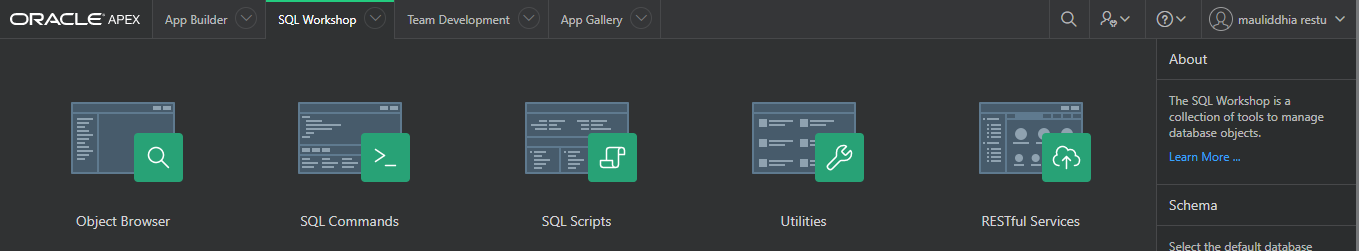
\includegraphics[scale=0.28]{figures/13.PNG}
    \caption{Pembuatan Aplikasi}
    \label{aplikasi1}
\end{figure}
\item Lalu pilih add page seperti pada gambar \ref{aplikasi2}
\begin{figure}[!htbp]
    \centering
    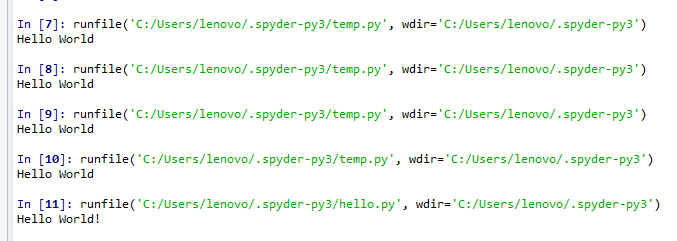
\includegraphics[scale=0.28]{figures/12.PNG}
    \caption{Pembuatan Aplikasi}
    \label{aplikasi2}
\end{figure}
\item Beri nama dan pilih tabel yang mau dimasukkan, tampilan tabel bisa berupa interactive report, diagram dan lain lain sesuai selera jika sudah jangan lupa centang include form agar kita bisa memasukkan data dari aplikasi tersebut seperti pada gambar \ref{aplikasi3} dan \ref{aplikasi4}
\begin{figure}[!htbp]
    \centering
    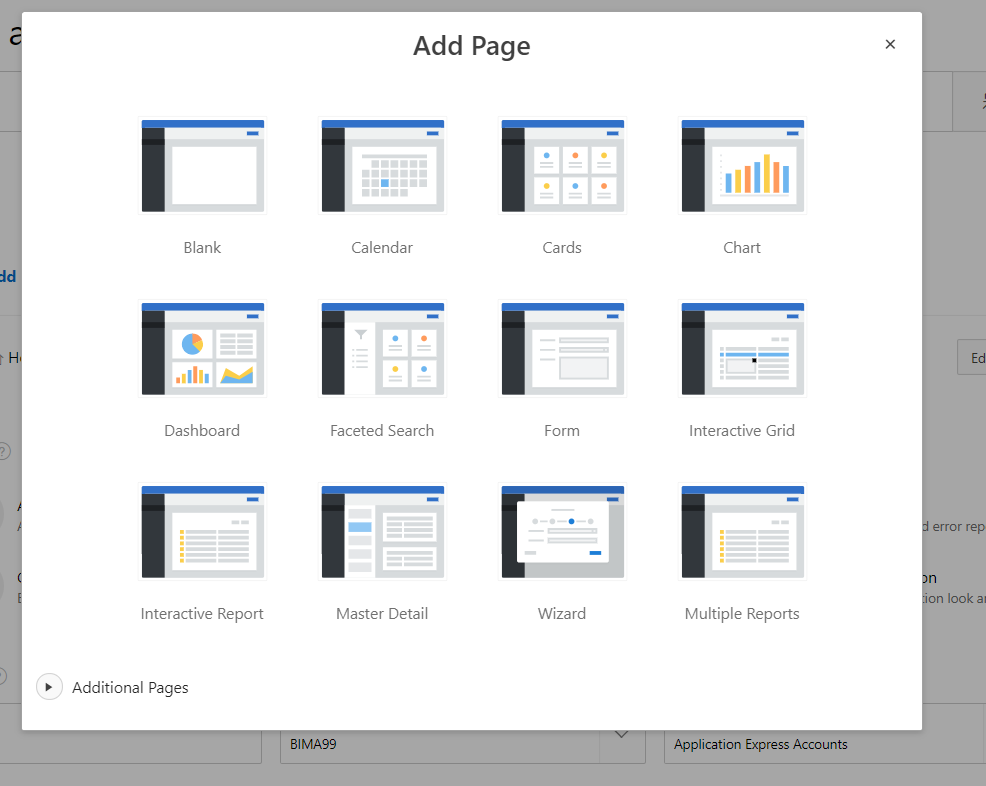
\includegraphics[scale=0.28]{figures/14.PNG}
    \caption{Pembuatan Aplikasi}
    \label{aplikasi3}
\end{figure}
\begin{figure}[!htbp]
    \centering
    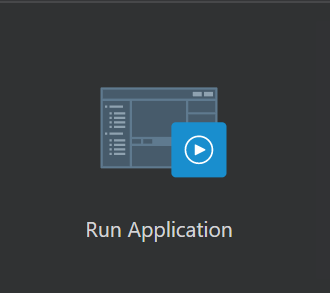
\includegraphics[scale=0.25]{figures/15.PNG}
    \caption{Pembuatan Aplikasi}
    \label{aplikasi4}
\end{figure}
\item Lalu buat satu data untuk bisa melihat semua data yang ada seperti misalnya halaman Admin formnya adalah master detail dan tabel yang dipilih adalah tabel utama yang berelasi dengan semua tabel seperti pada gambar \ref{aplikasi5}
\begin{figure}[!htbp]
    \centering
    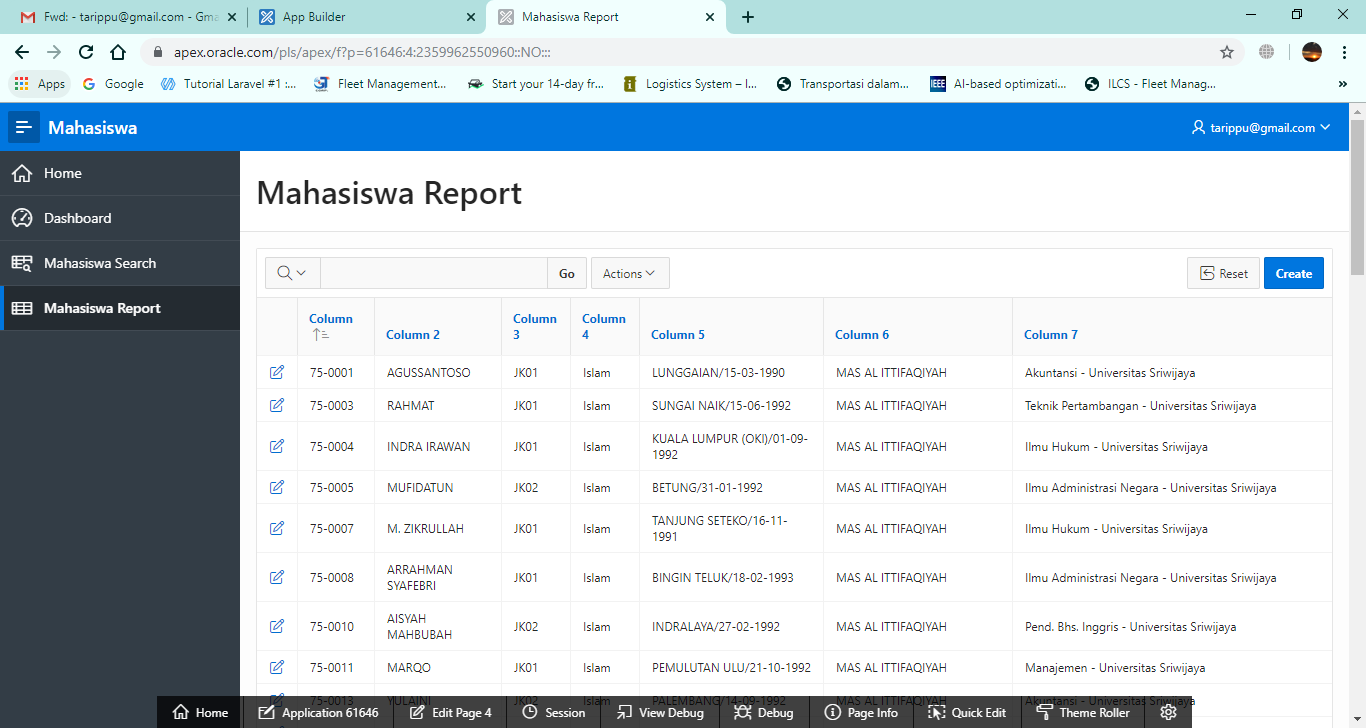
\includegraphics[scale=0.25]{figures/16.PNG}
    \caption{Pembuatan Aplikasi}
    \label{aplikasi5}
\end{figure}
\item Tunggu loading pembuatan aplikasinya seperti pada gambar \ref{aplikasi6}
\begin{figure}[!htbp]
    \centering
    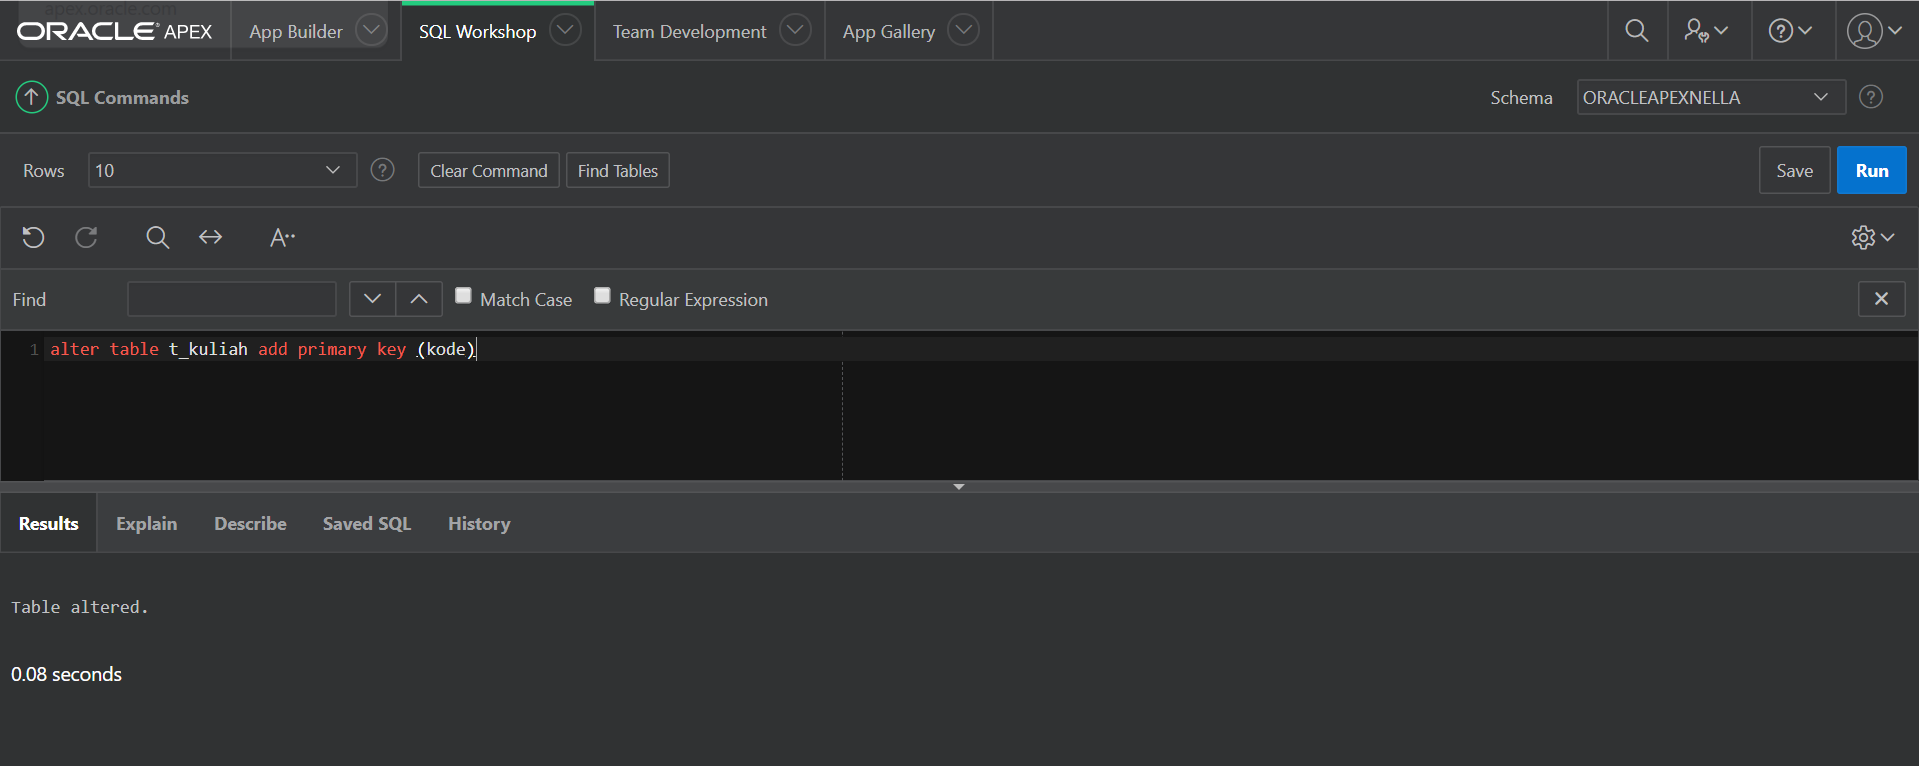
\includegraphics[scale=0.28]{figures/17.PNG}
    \caption{Pembuatan Aplikasi}
    \label{aplikasi6}
\end{figure}
\item Setelah terbuat maka kalian bisa menginsert, update, atau delete dan datanya akan terecord di history pelanggan seperti pada gambar \ref{aplikasi7}
\begin{figure}[!htbp]
    \centering
    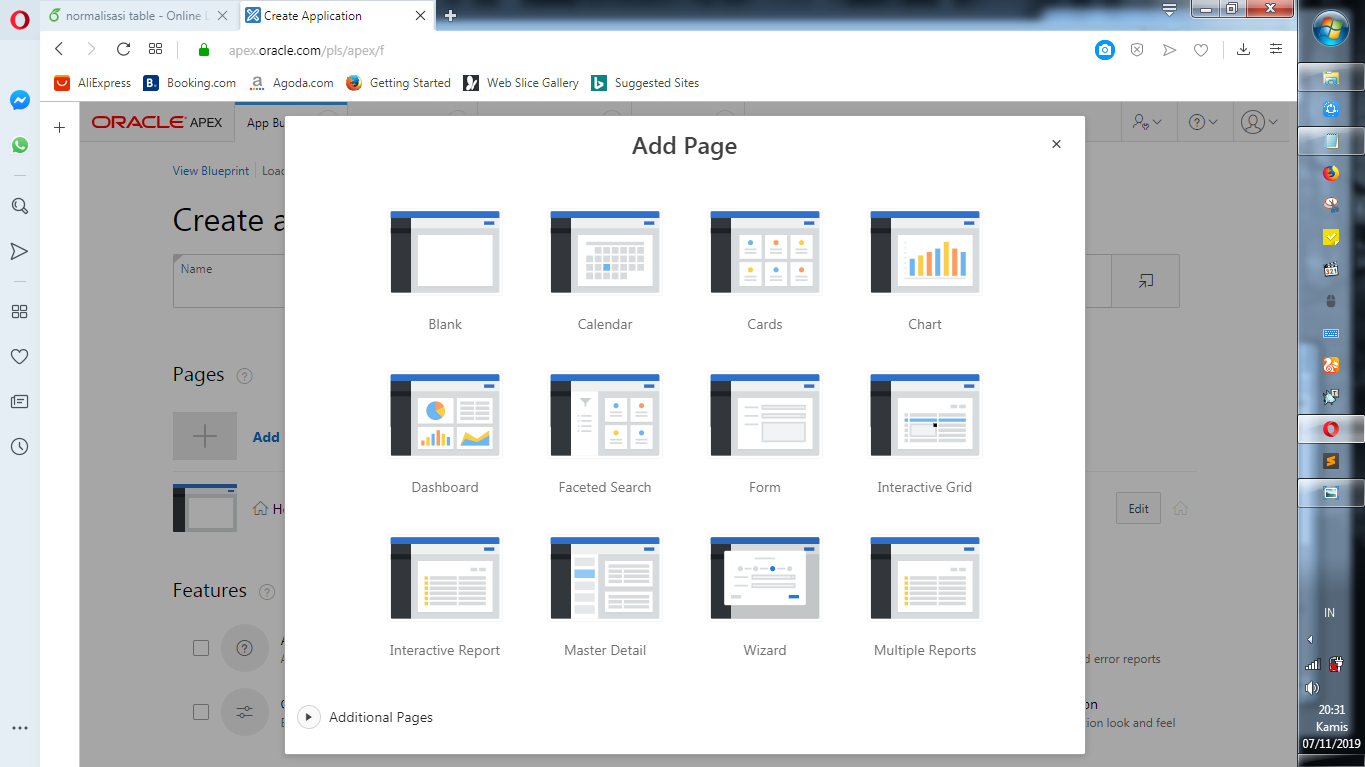
\includegraphics[scale=0.28]{figures/18.PNG}
    \caption{Pembuatan Aplikasi}
    \label{aplikasi7}
\end{figure}
\end{itemize}

\section{Workspace, Email, dan Password Oracle Apex}
\begin{itemize}
    \item ORACLE\_DIMAS
    \item dimas.maulana370@gmail.com
    \item redial24
    \item link https://apex.oracle.com/pls/apex/f?p=70540:LOGIN\_DESKTOP:100387812619614:::::
\end{itemize}
\end{document}

